\section{ニコ書を支えるAC5}

アーマードコアというゲームをご存知でしょうか?
様々な部位のパーツと武器を組み合わせてロボット(アーマードコア;AC)を作り、
敵のACと戦うゲームです。
最新作のAC5では、ネットワークを通してチーム対戦が可能で、
実際にACで戦う4人と、オペレータとして指示を出す1人と役割が分かれていて、
よりチームプレーが求められるゲームシステムになっています。

ニコ書チームはチームnicobookとしてAC5に参戦しました。

\begin{figure}[H]
\centering
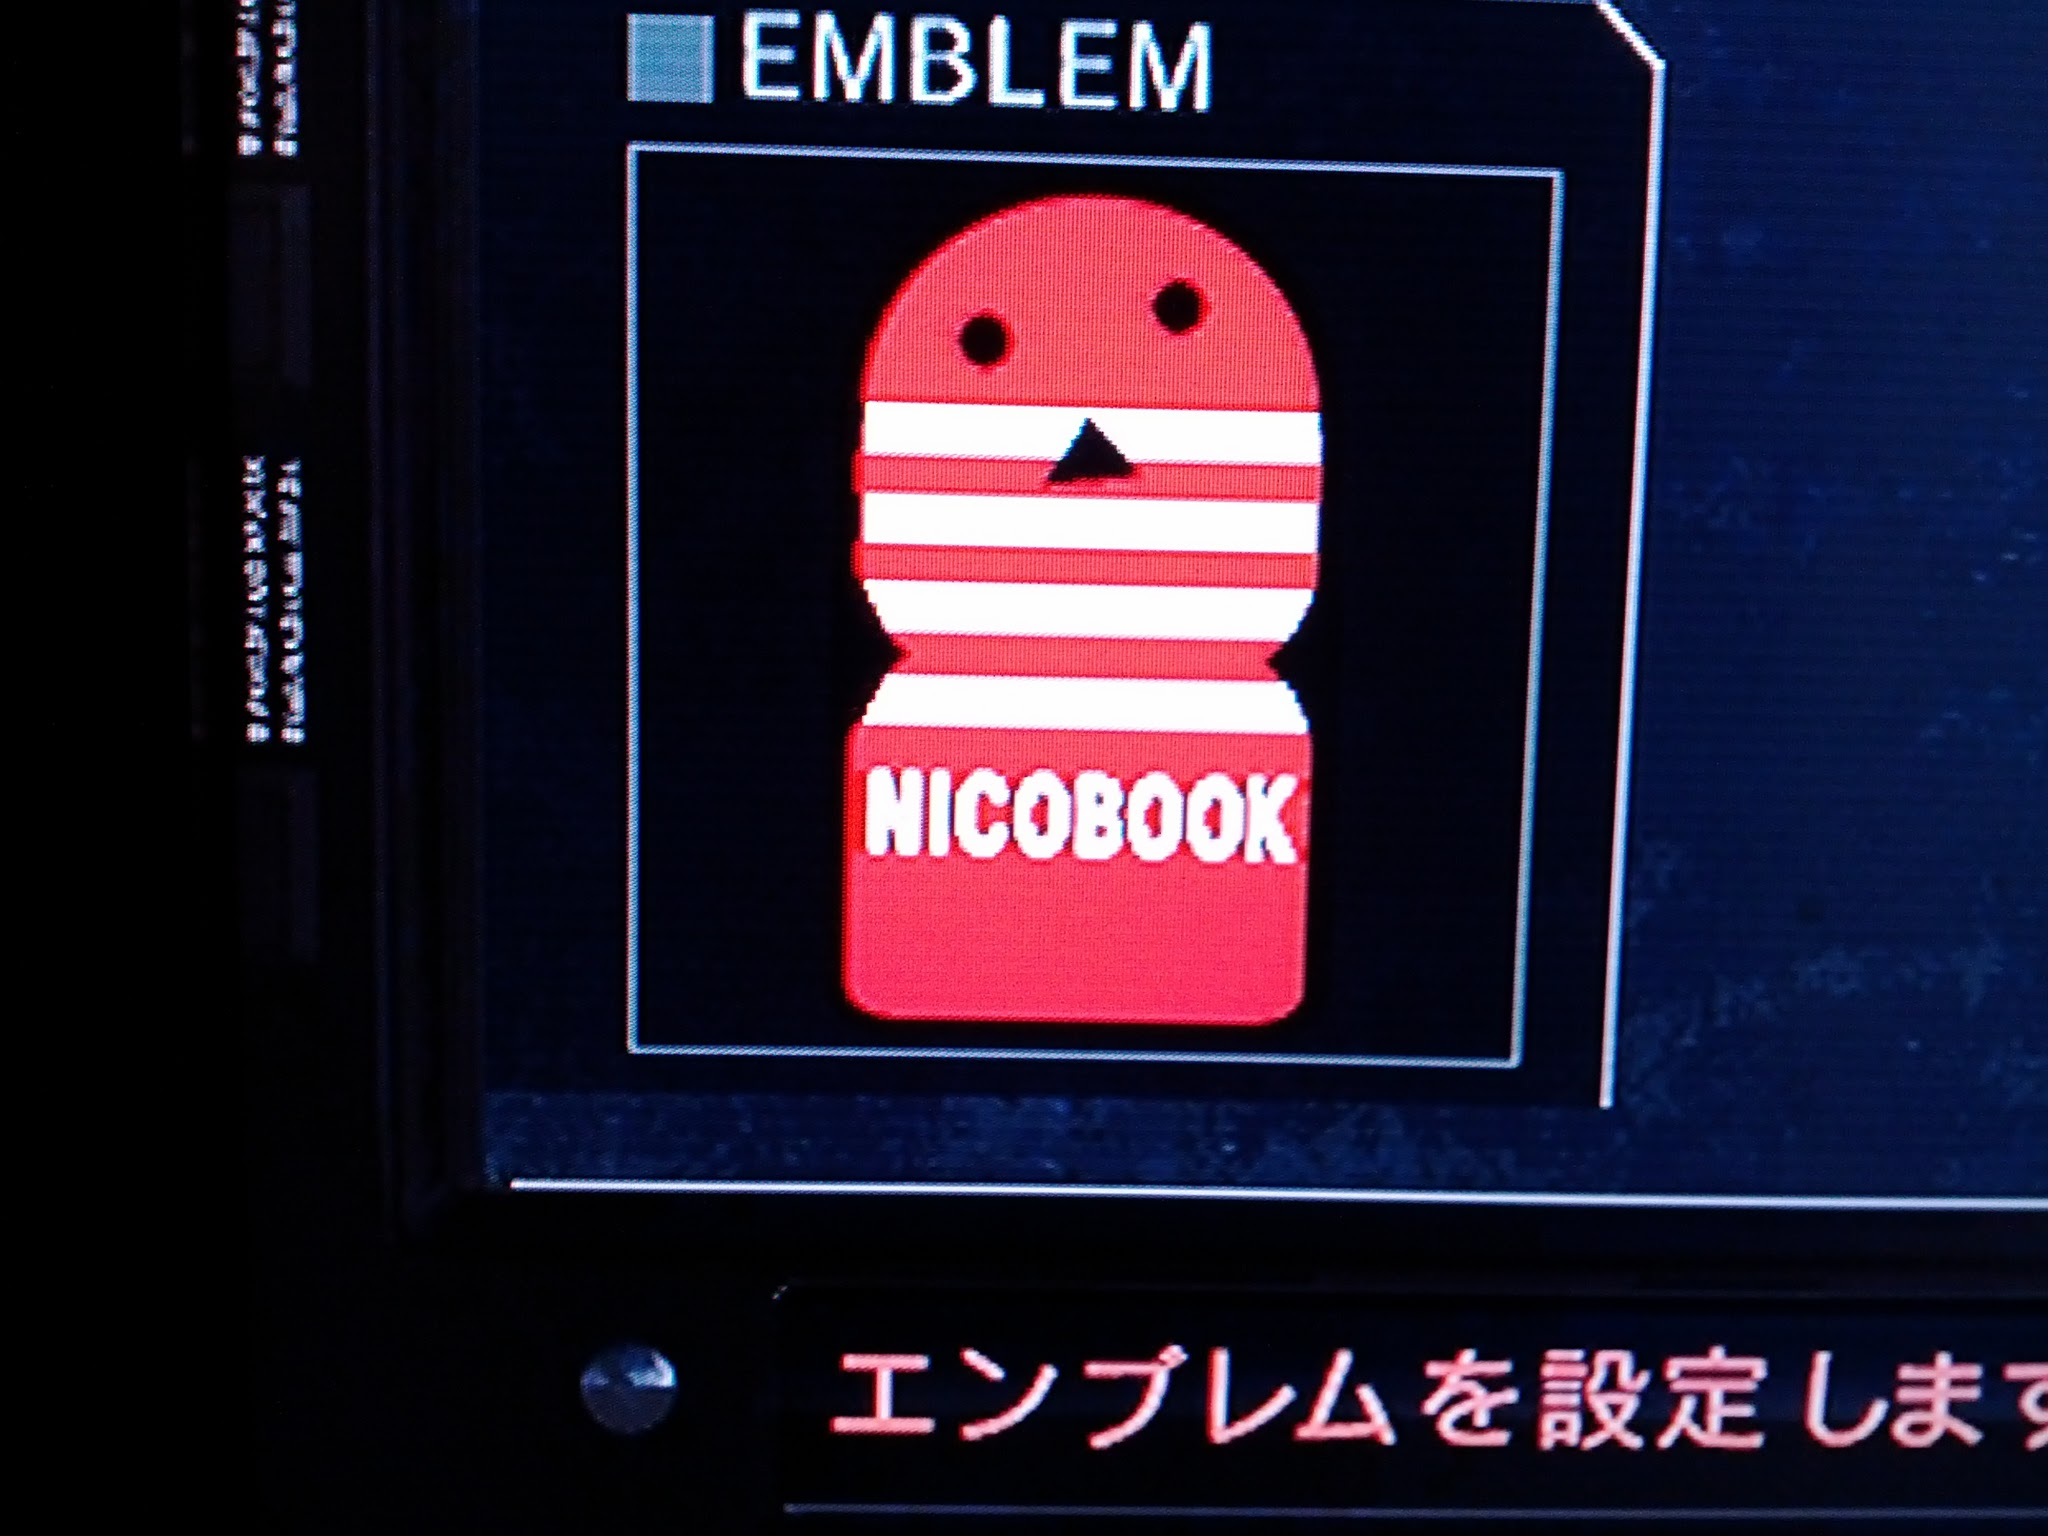
\includegraphics[width=0.6\textwidth]{../images/ac5_emb.jpg}
\caption{AC5エンブレム}
\end{figure}

\subsection{ニコ書チームを本当に支えたAC5}

AC5はネットゲームです。
対戦相手はネットワークの向こうにいる人間で、もちろん人間は生活のパターンがあります。
すなわち、対戦相手の多くは朝起き、仕事に行き、夜に帰り、少しゲームをして寝る、という真人間です。

ドワンゴという会社は基本的に出社時間は自由です。
しかし我々はAC5のためにコアタイムを設定しました。 \emph{23時から25時}
です。

え? なんかおかしいって? コアタイムのコアは \emph{もちろん}
アーマードコアのコアですよ?

23時から25時の間にアーマードコアに出社すると決めたことにより、 自然と
\emph{早く帰る} 習慣が生まれました。
しかし、早く帰ることにより労働時間が短くなる結果、
想定していた開発工数が取れなくなるのではないかという懸念がありました。
この懸念に対し我々は、減った時間を捻出するために \emph{早く来る}
という革命的ライフハックを発明し、 問題を解決しました。

つまり一言で言うと \emph{真人間に近づいたの} のです。

\subsection{リアル ブリーフィング}

ニコ書チームはAC5にもKPTを導入しました。
毎週、振り返りMTGを社内の一番広い会議室に設定し、
様々な出前を注文し、夕食を食べながらAC5の戦術について真剣に話し合いました。

\subsection{ニコ書を支えなかった Diablo III}

あれは廃人しか産みませんでした。
